\documentclass{beamer}
\usepackage{ctex, hyperref}
\usepackage[T1]{fontenc}

% other packages
\usepackage{latexsym,amsmath,xcolor,multicol,booktabs,calligra}
\usepackage{graphicx,pstricks,listings,stackengine}

\author{田凯夫、袁方舟}
\title{期末项目展示}
\subtitle{NaiveFS}
\institute{清华大学计算机科学与技术系}
\date{2022年6月8日}
\usepackage{Tsinghua}

% defs
\def\cmd#1{\texttt{\color{red}\footnotesize $\backslash$#1}}
\def\env#1{\texttt{\color{blue}\footnotesize #1}}
\definecolor{deepblue}{rgb}{0,0,0.5}
\definecolor{deepred}{rgb}{0.6,0,0}
\definecolor{deepgreen}{rgb}{0,0.5,0}
\definecolor{halfgray}{gray}{0.55}

\lstset{
    basicstyle=\ttfamily\small,
    keywordstyle=\bfseries\color{deepblue},
    emphstyle=\ttfamily\color{deepred},    % Custom highlighting style
    stringstyle=\color{deepgreen},
    numbers=left,
    numberstyle=\small\color{halfgray},
    rulesepcolor=\color{red!20!green!20!blue!20},
    frame=shadowbox,
}


\begin{document}

\kaishu
\begin{frame}
    \titlepage
    \begin{figure}[htpb]
        \begin{center}
            
\includegraphics[width=0.2\linewidth]{pic/Tsinghua_University_Logo.eps}
        \end{center}
    \end{figure}
\end{frame}

\begin{frame}
    \tableofcontents[sectionstyle=show,subsectionstyle=show/shaded/hide,subsubsectionstyle=show/shaded/hide]
\end{frame}


\section{项目背景}

\begin{frame}{FUSE}
    \begin{itemize}[<+-| alert@+>] % 当然,除了alert,手动在里面插 \pause 也行
        \item FUSE(Filesystem In Userspace)是一个面向类Unix计算机操作系统的软件接口
        \item 提高开发效率,简化在内核中实现文件系统的工作量
        \item 在用户态实现文件系统会引入额外的特权级切换带来的开销
    \end{itemize}
\end{frame}

\begin{frame}{EXT2}
    \begin{itemize}[<+-| alert@+>] % 当然,除了alert,手动在里面插 \pause 也行
        \item Linux上的第一款商业级文件系统
        \item 规范较为简单,便于实现和扩展
    \end{itemize}
\end{frame}


\section{实现思路}

\begin{frame}{总体架构}

\begin{figure}[htpb]
    \centering
    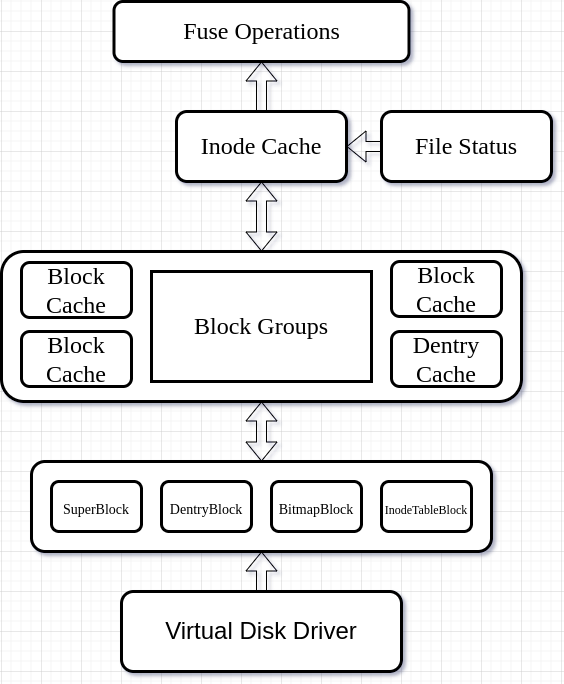
\includegraphics[width=0.5\linewidth]{pic/img.drawio.png}
    \caption{总体架构}
\end{figure}

\end{frame}

\begin{frame}{\textbf{Block}}
\begin{itemize}[<+-| alert@+>]
    \item 各种Block的基类
    \item Block默认大小为\textbf{4096B},在创建时会分配内存空间,在删除时释放分配的内存空间
    \item 处理创建Block时可能的两种情况:1.Block可能是新创建的,虚拟磁盘中的这块区域还未被使用过;2.Block从虚拟磁盘中读取过去写入的数据
    \item 提供flush操作,将Block中的数据写入到虚拟磁盘对应的偏移量处
\end{itemize}
\end{frame}

\begin{frame}{\textbf{FileSystem}}
\begin{itemize}[<+-| alert@+>]
    \item 创建文件系统时会检查Super Block状态,如果未被初始化,就创建Root Inode作为根目录
    \item 查找:根据提供的路径向下查找,先检查Dentry Cache,再检查Dentry Block
    \item 创建:1.查询父目录并获取父目录的Inode;2.遍历Dentry Block;3.分配新的Inode
    \item 删除:减少引用计数,若引用计数归零,则删除Inode并清空Cache对应项
\end{itemize}
\end{frame}

\begin{frame}{\textbf{FileStatus}}
\begin{itemize}[<+-| alert@+>]
    \item 
\end{itemize}
\end{frame}

\begin{frame}{优化设计}
\begin{itemize}[<+-| alert@+>]
    \item \textbf{Dentry Cache}:多叉树结构,每一层采用环形链表,父节点指向最新被访问到的节点
    \item \textbf{Block Cache}:使用散列表对Block进行管理,采用LRU替换策略,Block的空间只有在被替换的时候才会释放
    \item \textbf{Inode Cache}:对多个FileStatus共用的inode进行缓存,用读写锁管理并发访问,更新时会同步更新引用它的FileStatus
\end{itemize}
\end{frame}

\section{拓展实现}

\begin{frame}{加密}

\end{frame}

\begin{frame}{权限检查}

\end{frame}

\begin{frame}
    \begin{center}
        {\Huge DEMO}
    \end{center}
\end{frame}

\section{计划进度}
\begin{frame}
    \begin{itemize}
        \item 搭建运行环境
        \item 实现底层功能
        \item 实现Fuse相关函数
        \item 测试、优化性能
        \item 拓展实现
    \end{itemize}
\end{frame}

\begin{frame}
    \begin{center}
        {\Huge\calligra Thanks!}
    \end{center}
\end{frame}

\end{document}